\section{Primary benchmark map and prediction ledger}

The comparison values used in this section follow representative CODATA, PDG, NuFIT, Planck, and birefringence references \cite{codata2022,pdg2025,nufit2025,planck2018,minamiKomatsu2020,eskilt2023,sullivan2025}. The snapshot policy is frozen at CODATA 2022 / NIST for $\alpha(0)$, PDG 2025 for particle-mass and weak-mixing rows, NuFIT 2025 for neutrino-angle rows, and Planck 2018 for the baryon-fraction reconstruction used here. The main-text table is intentionally restricted to six rows whose comparison language is already reasonably convention-complete. The compact mass surface is given separately in \Cref{tab:sm-mass-ledger-ew,tab:sm-mass-ledger-quarks}; more exploratory rows and the main unresolved comparison are moved to Appendix~\ref{app:benchmarks}. Beyond that narrow six-row surface, the manuscript also carries a small operational prediction set of experimentally actionable rows, collected explicitly below. The $\Omega_b$ row is a present-epoch reconstruction from the Planck pair $(\Omega_b h^2,H_0)$, not a claim that $\Omega_b(t)$ itself is a timeless seed quantity.
Here \enquote{carrier closure} abbreviates the self-consistent electromagnetic closure expression with explicit retained second-order opening $\phiztwo(\alpha)$ and term $\delta_2=\frac54\deltatop^2$. The $\alpha^{-1}(0)$ row is therefore structurally different from the four bridge rows $(\beta,\Omega_b,\lambda_C,\sin^2\theta_{13})$, which are all projections of the same retained seed $\phiz$.

\begin{table}[t]
\centering
\scriptsize
\setlength{\tabcolsep}{2pt}
\resizebox{\linewidth}{!}{%
\begin{tabular}{@{}llrrrrll@{}}
\toprule
\makecell[l]{Obs.} & \makecell[l]{TFPT\\formula} & \makecell[r]{TFPT\\value} & \makecell[r]{Exp.\\value} & \makecell[r]{Unc.} & \makecell[r]{Residual} & \makecell[l]{Scale /\\scheme} & Status \\
\midrule
$\alpha^{-1}(0)$ & \makecell[l]{self-consistent carrier closure\\$\phiztwo(\alpha)$ and $\delta_2$} & \num{137.0359992} & \num{137.03599918} & \num{2.1e-8} & $+1.87\sigma$ & \makecell[l]{Thomson\\on-shell} & Benchmark bridge \\
\makecell[l]{$\bar\alpha^{(5)}$\\$(M_Z)^{-1}$} & \makecell[l]{$\mathcal R_{\SM}$\\$[\alpha(0)]$} & \num{127.9405} & \num{127.93} & \num{0.008} & $+1.32\sigma$ & \makecell[l]{$\overline{\mathrm{MS}}$\\at $M_Z$} & Benchmark bridge \\
$\lambda_C$ & $\sqrt{\phiz(1-\phiz)}$ & \num{0.22438} & \num{0.22431} & \num{8.5e-4} & $+0.08\sigma$ & \makecell[l]{CKM\\proxy} & Benchmark bridge \\
$\sin^2\theta_{13}$ & \makecell[l]{$\phiz$\\$e^{-5/6}$} & \num{0.02311} & \num{0.02224} & \num{5.7e-4} & $+1.524\sigma$ & \makecell[l]{NuFIT\\NO} & Benchmark bridge \\
$\Omega_b$ & \makecell[l]{$(4\pi-1)$\\$\beta_{\mathrm{rad}}$} & \num{0.04894} & \num{0.04930} & \num{8.57e-4} & $-0.421\sigma$ & \makecell[l]{Planck 2018\\present epoch\\from $\Omega_b h^2$} & Benchmark bridge \\
$\beta$ & \makecell[l]{$\beta_{\mathrm{rad}}$\\in degrees} & \num{0.242} & \num{0.35} & \num{0.14} & $-0.77\sigma$ & \makecell[l]{Planck 2018\\Minami--Komatsu} & Benchmark bridge \\
\bottomrule
\end{tabular}}
\caption{Primary benchmark table for the main-text claims. Supplementary rows and out-of-sample checks are collected in Appendix~\ref{app:benchmarks}.}
\label{tab:benchmark}
\end{table}

\begin{remark}[One seed, four projections]
The bridge rows are not statistically independent hits. With
\[
\beta_{\mathrm{rad}}=\frac{\phiz}{4\pi},
\qquad
\Omega_b=(4\pi-1)\beta_{\mathrm{rad}},
\qquad
\lambda_C=\sqrt{\phiz(1-\phiz)},
\qquad
\sin^2\theta_{13}=\phiz e^{-\gamma},
\]
the four-row map is a one-variable seed map
\[
\mathcal S(\phiz):=\bigl(\beta_{\mathrm{rad}},\Omega_b,\lambda_C,\sin^2\theta_{13}\bigr),
\]
with Jacobian
\[
\frac{d\mathcal S}{d\phiz}
=
\left(
\frac{1}{4\pi},
\,
1-\frac{1}{4\pi},
\,
\frac{1-2\phiz}{2\sqrt{\phiz(1-\phiz)}},
\,
e^{-\gamma}
\right).
\]
Thus $\beta$, $\Omega_b$, $\lambda_C$, and $\sin^2\theta_{13}$ are one seed and four shadows, not four detached benchmark events. They remain in the table because their comparison conventions and uncertainty models differ, not because the underlying algebraic source is independent.
\end{remark}

\subsection{Operational prediction set}

The six-row benchmark table is not the whole experimental surface of the manuscript. \Cref{tab:operational-prediction-set} collects the rows that are operationally testable on near- to medium-term timescales, while keeping their status, next test, kill criterion, and dependency structure explicit. The point is not to flatten them into one truth class. Rather, the \emph{Status} column keeps the manuscript's global truth-mode vocabulary, while the derivation and dependency columns show which rows are benchmark-bridge outputs, which belong only to retained branch selections, which are closure consequences, and which rely on downstream scale grammar. The electroweak triple $(m_W,\hat s_Z^2,\alpha_s)$ is intentionally \emph{not} promoted here yet: the local carrier closure is fixed, but the remaining branch sensitivity still sits in the declared matching functionals $\mathcal R_{\SM}^{\mathrm{match}}$, so these rows are better kept out of the compact operational set.

\begin{table}[t]
\centering
\tiny
\sisetup{round-mode=none, group-minimum-digits=20}
\setlength{\tabcolsep}{0.8pt}
\renewcommand{\arraystretch}{0.95}
\sloppy
\resizebox{\linewidth}{!}{%
\begin{tabular}{@{}>{\raggedright\arraybackslash}p{0.12\linewidth}>{\raggedright\arraybackslash}p{0.17\linewidth}>{\raggedright\arraybackslash}p{0.09\linewidth}>{\raggedright\arraybackslash}p{0.13\linewidth}>{\raggedright\arraybackslash}p{0.12\linewidth}>{\raggedright\arraybackslash}p{0.17\linewidth}>{\raggedright\arraybackslash}p{0.11\linewidth}@{}}
\toprule
\makecell[l]{Observable} & \makecell[l]{TFPT\\target} & Status & \makecell[l]{Derivation\\source} & \makecell[l]{Next\\test} & \makecell[l]{Kill\\criterion} & \makecell[l]{Dependency\\class} \\
\midrule
\makecell[l]{Cosmic\\birefringence $\beta$} & \num{0.2424}$^\circ$ & \makecell[l]{Benchmark\\bridge} & seed map $\beta=\phiz/(4\pi)$ & \makecell[l]{calibrated CMB\\rotation analysis} & \makecell[l]{calibrated $\beta=0$\\within $\pm \num{0.05}^\circ$} & seed \\
$\delta_{\mathrm{CKM}}$ & \makecell[l]{\num{1.198}\\rad} & \makecell[l]{Benchmark\\bridge} & \makecell[l]{holonomy triangle /\\phase lattice} & \makecell[l]{global flavor\\fit} & \makecell[l]{exclusion at\\$\ge 3\sigma$} & \makecell[l]{flavor\\bridge} \\
\makecell[l]{Rare kaons\\$K\to\pi\nu\bar\nu$} & \makecell[l]{$\mathrm{BR}(K^+)$\\$=\num{8.22e-11}$\\$\mathrm{BR}(K_L)$\\$=\num{2.65e-11}$} & \makecell[l]{Benchmark\\bridge} & \makecell[l]{CKM point in\\short-distance\\amplitudes} & \makecell[l]{NA62 / KOTO\\program} & \makecell[l]{$K^+$ outside\\$[6,10]\times10^{-11}$\\or $K_L$ mismatch} & \makecell[l]{flavor\\bridge} \\
\makecell[l]{PMNS phase /\\octant} & \makecell[l]{$\delta_{\mathrm{CP}}=240^\circ$\\$\sin^2\theta_{23}=\num{0.4557}$} & \makecell[l]{Conditional\\extension} & \makecell[l]{oscillation\\branch /\\phase lattice} & \makecell[l]{global oscillation\\fit} & \makecell[l]{exclude $240^\circ$\\or lower octant\\at $\ge 3\sigma$} & \makecell[l]{neutrino\\branch} \\
$\Sigma m_\nu$ & \makecell[l]{\num{5.8764e-2}\\eV} & \makecell[l]{Conditional\\extension} & \makecell[l]{oscillation\\branch\\(NO)} & \makecell[l]{cosmological\\mass-sum analyses} & \makecell[l]{robust upper bound\\below the branch value} & \makecell[l]{neutrino\\branch} \\
$m_{\beta\beta}$ & \makecell[l]{\num{1.516e-3}\\eV} & \makecell[l]{Conditional\\extension} & \makecell[l]{Majorana lattice\\on oscillation\\branch} & \makecell[l]{light-Majorana\\$0\nu\beta\beta$ searches} & \makecell[l]{detection implying\\$m_{\beta\beta}\gtrsim \num{1e-2}$ eV} & \makecell[l]{neutrino\\branch} \\
\makecell[l]{nEDM / strong\\CP} & $\bar\theta=0$ & Closure & \makecell[l]{admissibility-side\\strong-CP theorem} & \makecell[l]{next-gen EDM\\searches} & \makecell[l]{stable nonzero\\hadronic EDM signal} & closure \\
\makecell[l]{Axion haloscope\\window} & \makecell[l]{$m_a\approx \num{65.19}$\\$\mu\mathrm{eV}$\\$\nu_a\approx \num{15.764}$\\$\mathrm{GHz}$} & \makecell[l]{Conditional\\extension} & \makecell[l]{PQ block /\\scale grammar} & \makecell[l]{haloscope scan\\near \num{15.764} GHz} & \makecell[l]{exclusion in\\\num{15.764} GHz\\$\pm \num{50}$ MHz} & \makecell[l]{scale\\grammar} \\
\bottomrule
\end{tabular}}
\caption{Operational prediction set with explicit status and dependency classes.}
\label{tab:operational-prediction-set}
\end{table}

\begin{remark}[Independence classes]
The rightmost column in \Cref{tab:operational-prediction-set} records dependency structure rather than truth value, using deliberately compact class labels. \emph{Seed} means a row is a projection of the retained scalar seed $\phiz$; \emph{flavor bridge} means it is downstream of the CKM/PMNS transport bridge; \emph{neutrino branch} means it belongs to the retained oscillation branch or to the separate seesaw-side cross-check layer; \emph{closure} means it is a direct consequence of an admissibility-closure theorem; and \emph{scale grammar} means it appears only after the optional PQ / E$_8$ ladder is granted. This keeps statistical and logical non-independence visible at the same place where the experimental targets are listed.
\end{remark}

\subsection{Compact prediction ledger}

The main benchmark table shows only a narrow comparison surface. To keep the compiler structure visible, \Cref{tab:prediction-ledger} summarizes which output packages belong to which layer of the paper.

\begin{table}[t]
\centering
\small
\begin{tabularx}{\linewidth}{@{}>{\raggedright\arraybackslash}p{0.18\linewidth}>{\raggedright\arraybackslash}p{0.12\linewidth}YY@{}}
\toprule
Domain & Status & Output package & Source layer \\
\midrule
Carrier packet & Hard & $E_3\oplus E_2$, $G_{\SM}^{\mathrm{glob}}$, $S^+$, $\gamma$, $\bone(N_{\mathrm{fam}},N_\Phi)$ & minimal carrier theorem and half-spinor decomposition \\
Kernel constants & Hard / retained & $\cthree$, $\phibase$, $\phiz$, $\deltatop$ & hard constants plus retained canonical seed in the carrier-form closure equation \\
Family / occupancy layer & Closure & $\Padm$, $F$, $\Oadm=48$, $\deltatop$ & APS family closure and occupancy corollary \\
Geometric compiler & Closure & $\Phi$, $\Mpl$, $\vgeo$, $R^2$ channel & bosonic index plus relative heat-kernel closure \\
Transport compiler & Closure / retained rule & $Y_f$, $m_f$, CKM, PMNS & matrix holonomy theorem together with retained path-length grammar \\
QCD closure & Closure & $\Hhad$, anomaly inflow, $\bar\theta=0$ & singlet admissibility plus positive-kernel hardening \\
Benchmark bridge & Benchmark bridge & $\mathcal R_{\SM}$, $\alpha$, $\beta$, $\lambda_C$, thresholds, ledgers & scheme-complete comparison layer \\
Downstream ladder & Conditional extension & E$_8$ scale ratios and inflation-side imports & optional appendix-level scale grammar \\
Record layer & Closure & $\Arec$, $\Aobs$, $\Pred$ & admissible gap plus observer-algebra definition \\
Horizon layer & Conditional extension & modular inner-seam language & appendix-level extension \\
\bottomrule
\end{tabularx}
\caption{Compact prediction ledger for the carrier-first compiler presentation after the closure layer is separated from the benchmark bridge.}
\label{tab:prediction-ledger}
\end{table}

\subsection{Realism audit of the present compiler surface}

The present comparison surface is deliberately uneven, and that unevenness is informative rather than embarrassing. Carrier algebra and the self-consistent $\alpha$ row are the sharpest parts of the manuscript. The seed-driven bridge rows are useful because they are transparent and mutually constrained, not because they are independent. In the mass sector, the manuscript should be read as a mixed surface: some rows are genuinely derived, some are explicit candidates, and some are anchor-dependent by construction. The charged-lepton candidates remain visibly softer than the best kernel-linked rows, while the light-quark and hadronic checks show that the transport side is already more than rhetorical. The neutrino block is now displayed explicitly in two layers: oscillation-inversion branch values for the operational rows and a separate seesaw-side geometric cross-check through $M_R$. In the gauge sector, the local carrier closure is now explicit, while the remaining branch sensitivity is isolated in the declared seam and Wilson matching functionals. The right summary is therefore not that the full compiler is finished, but that the hard core is strong, the comparison map is explicit, and the remaining theorem load is localized.

\subsection{Residual map and principal comparison refinements}

The residuals for the restricted six-row table are shown in \Cref{fig:residual-plot}. The carrier-linked electromagnetic, birefringence, and baryon-density channels all remain within the displayed few-sigma window. The CKM phase is not plotted here because it is better treated, at present, in the operational prediction set and Appendix~\ref{app:benchmarks} rather than inside the restricted six-row residual plot.

\begin{figure}[t]
\centering
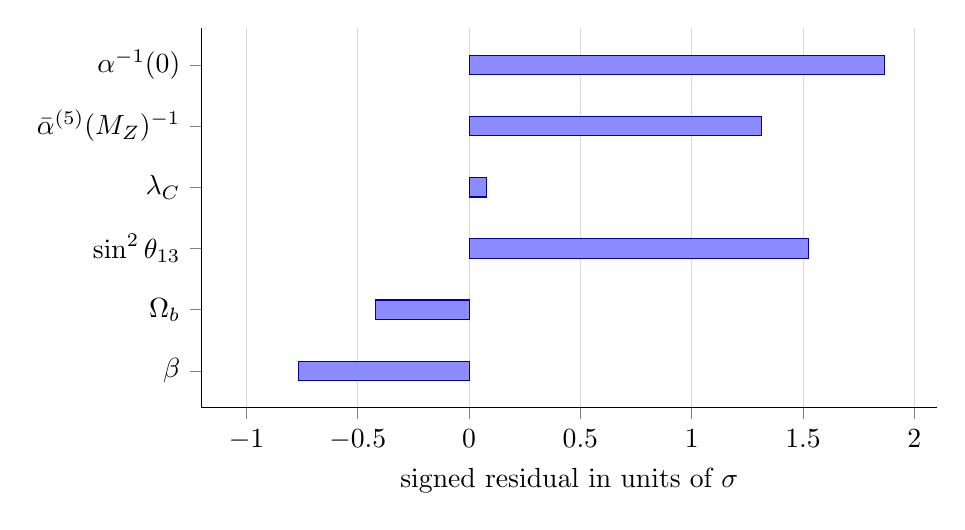
\begin{tikzpicture}
\begin{axis}[
    width=0.9\linewidth,
    height=6.4cm,
    xbar,
    bar width=7pt,
    xmin=-1.2,
    xmax=2.1,
    xlabel={signed residual in units of $\sigma$},
    symbolic y coords={beta,omegab,theta13,lambdac,alphaMZ,alpha0},
    ytick=data,
    yticklabels={$\beta$,$\Omega_b$,$\sin^2\theta_{13}$,$\lambda_C$,$\bar\alpha^{(5)}(M_Z)^{-1}$,$\alpha^{-1}(0)$},
    enlarge y limits=0.12,
    axis x line*=bottom,
    axis y line*=left,
    tick align=outside,
    major grid style={draw=gray!30},
    xmajorgrids=true
]
\addplot[fill=blue!45, draw=blue!70!black] coordinates {
    (-0.768,beta)
    (-0.421,omegab)
    (1.524,theta13)
    (0.078,lambdac)
    (1.315,alphaMZ)
    (1.865,alpha0)
};
\end{axis}
\end{tikzpicture}
\caption{Residual plot for the main benchmark rows with declared uncertainties.}
\label{fig:residual-plot}
\end{figure}

The principal remaining refinements are therefore specific rather than diffuse:
\begin{itemize}[leftmargin=1.5em, topsep=3pt, itemsep=2pt]
    \item the CKM phase is resolved to second transport order through the holonomy triangle phase, with only the $O(\lambda_C^4)$ transport remainder left outside the main text,
    \item the nonabelian comparison channels now split into fixed local carrier closure and explicit matching functionals, so the remaining sensitivity is branch-side rather than structural,
    \item direct-search interface rows remain pressure tests on the closed branch rather than precision residual rows.
\end{itemize}

\subsection{Falsification matrix}

The present draft does not ask the reader to accept one undifferentiated \enquote{compiler} claim. Each main-text closure statement has a corresponding local or global failure mode, and those failure modes should be readable without first decoding the appendix tables.

The matrix below is therefore intentionally short. It collects only the load-bearing main-paper statements whose failure would break the carrier-first architecture at the theorem level, rather than every downstream benchmark row or optional appendix interface.

\begin{table}[t]
\centering
\small
\begin{tabularx}{\linewidth}{@{}>{\raggedright\arraybackslash}p{0.24\linewidth}YY>{\raggedright\arraybackslash}p{0.13\linewidth}@{}}
\toprule
Statement & What would falsify it & Sector affected & Local or global failure \\
\midrule
Primitive relative spectral dynamics & ill-posed APS domain or no finite admissible spectral action on the retained branch & Hard / closure & global \\
Minimal carrier $E_3\oplus E_2$ & failure to recover the one-family packet or the global quotient from the carrier theorem & Hard & global \\
APS family closure and $\Oadm=48$ & failure of the APS family theorem to globalize the local count & Closure & local-to-structural \\
Bosonic relative index selecting $\Phi$ & no unique seam-even doublet or an unavoidable extra light triplet & Closure & local \\
local spectral-scale / gravity closure for $\Mpl$ and $\vgeo$ & inability to obtain one common closure for $\Mpl$, $\vgeo$, the Einstein branch, and the $R^2$ branch & Closure & global \\
Transport / strong-CP closure & nonzero determinant phase or an unavoidable $\bar\theta$ counterterm & Closure & local \\
Confinement as admissible word selection & necessity of physical states with $z(w)\neq1$ in the low-energy spectrum & Closure & local \\
Nonperturbative admissible QFT closure & no admissible mass gap or no clustering on the retained branch & Closure & global \\
\bottomrule
\end{tabularx}
\caption{Falsification matrix for the present main-paper claims.}
\label{tab:falsification}
\end{table}

\section{Compiler theorem and benchmark bridge}

\subsection{Compiler chain}

Collecting the present primitive layer, the hard carrier kernel, the closure theorems from the admissibility complex, and the benchmark bridge, the compiler line is
\begin{equation}
\label{eq:conditional-compiler-chain}
\begin{aligned}
\Tprim
&\Rightarrow
(E_3\oplus E_2,\ G_{\SM}^{\mathrm{glob}},\ S^+)\\
&\Rightarrow
( \Padm,\ N_{\mathrm{fam}}=3,\ F,\ \Oadm=48,\ \Phi)\\
&\Rightarrow
( \Mpl,\ \vgeo,\ Y_f,\ \Hhad,\ \bar\theta )\\
&\Rightarrow
(m_f,\ V_{\mathrm{CKM}},\ U_{\mathrm{PMNS}},\ \Lambda_{\Seam,\mathrm{ren}})\\
&\Rightarrow
(\text{benchmarks},\ \Pred).
\end{aligned}
\end{equation}
This line is not meant as a slogan. Each arrow is attached either to a hard theorem, to one of the closure theorems of \Cref{sec:closure-theorems}, or to the declared benchmark bridge.

\subsection{Compiler theorem from the admissibility complex}

\begin{theorem}[Compiler theorem from the admissibility complex]
Assume the primitive and hard layers summarized in \Cref{tab:status-matrix}, together with the closure theorems of \Cref{sec:closure-theorems} and the declared benchmark bridge $\mathcal R_{\SM}$. Then every main-text observable in scope is classified by exactly one of the following modes:
\begin{enumerate}[label=(\roman*), leftmargin=1.5em, topsep=3pt, itemsep=2pt]
    \item a derived carrier or closure output,
    \item a retained branch value,
    \item an anchor-governed comparison image under $\mathcal R_{\SM}$,
    \item or a conditional downstream output.
\end{enumerate}
\end{theorem}

\begin{proof}[Proof sketch]
The proof is compositional. The primitive layer fixes the undecomposed relative spectral seed. The hard layer then fixes the carrier, the global Standard Model quotient, one family packet, the carrier norm, the abelian index, and the electromagnetic closure equation. The closure layer turns admissibility into an operative selector, globalizes the family theorem through $\APSfam$ data, selects the unique light Higgs mode, closes the local spectral-scale channel, lifts transport into a matrix-holonomy mass grammar with retained admissible transport packets, fixes the hadronic space and the strong-CP/anomaly sector, and reconstructs Lorentzian dynamics, record observables, and the admissible vacuum. The benchmark bridge finally translates this closed compiler surface into scheme-specified observables at the declared matching point. What remains outside these three layers is explicitly marked as conditional downstream output rather than silently promoted to a derived theorem.
\end{proof}

\subsection{Closure stack and benchmark bridge}

The compiler theorem above is only meaningful if the closure arrows are visibly attached to concrete input packages, output packages, and status labels. Otherwise the theorem reads like a slogan instead of a compressed map of the argument.

The following table is therefore the structural companion to the theorem: it records which objects belong to the closure stack proper, which objects belong only to the benchmark bridge, and how the paper expects those layers to interact.

\begin{table}[t]
\centering
\small
\begin{tabularx}{\linewidth}{@{}>{\raggedright\arraybackslash}p{0.20\linewidth}>{\raggedright\arraybackslash}p{0.18\linewidth}>{\raggedright\arraybackslash}p{0.20\linewidth}YY@{}}
\toprule
Closed statement & Input data & Output package & Status note & Benchmark role \\
\midrule
Primitive relative spectral dynamics & $X$, $D_{\mathrm{rel}}$, $f$, $\chiseed$, $\Delta\eta_\Sigma$ & well-posed primitive Euclidean seed & primitive datum & fixes the starting dynamics before carrier and closure are derived \\
Operative selector $\Padm$ & admissibility complex $(Q_{\mathrm{adm}},\Delta_{\mathrm{adm}},\Kadm)$ & sector selector for Higgs / QCD / CP & closed from admissibility complex & stabilizes all later sector statements \\
APS family closure & $\Seam$, $C_1,C_2,C_T$, $\APSfam$ data & $F$, $N_{\mathrm{fam}}=3$, $\Oadm=48$ & imported master theorem + closure compatibility & fixes flavor multiplicity globally \\
Bosonic and local spectral-scale closure & $E_3\oplus E_2$, $\mathcal B_{\mathrm{rel}}$, $\mathbb A_{\Seam}$, $E_{\mathrm{rel}}$, $Z_H$, $w_H$ & $\Phi$, $\Mpl$, $\vgeo$, gravity/cosmology branch & closed from admissibility complex & Higgs and scale sector are internally closed \\
Transport holonomy grammar & $U_6$, $D_y$, $\epsilon_f$, $\nabla_F$, admissible lengths & $Y_f$, $m_f$, CKM, PMNS & closure plus retained transport rule & sharp transport-side mass grammar \\
Hadronic / anomaly / strong-CP closure & $\Asing$, $\eta$ term, sheet exchange & $\Hhad$, $I_6^{\mathrm{tot}}=0$, $\bar\theta=0$ & closed from admissibility complex & QCD consistency and null-EDM route \\
Gap / clustering closure & $\epsilon_f$, $m_-$, $m_3$ & $m_*>0$, exponential clustering & closed from admissibility complex & nonperturbative QFT closure becomes explicit \\
OS / Lorentz / vacuum / record closure & $Z_{\mathrm{rel}}$, $\Theta$, $\Hrel$, $\Vadm$ & Lorentzian Hamiltonian, $\rho^\ast$, $\Lambda_{\Seam,\mathrm{ren}}$, $\Arec$, $\Pred$ & closed from admissibility complex & causal dynamics, record sector, and vacuum energy map \\
Wilson area-law route & $\chi_{\QCD}$, center-neutral Wilson functional & area-law confinement and no colored asymptotic states & conditional conjecture & turns the confinement route into a sharper strong-coupling statement \\
Comparison map $\mathcal R_{\SM}$ and retained $\delta_{\mathrm{ph}}$ saddle & $\alpha(0)$, thresholds, scheme map, observable map & benchmarks, residuals, ledgers & benchmark bridge & theory-versus-data translation becomes convention-complete \\
\bottomrule
\end{tabularx}
\caption{Closure stack and benchmark bridge for the present main-paper form.}
\label{tab:proof-obligations}
\end{table}

\section{Conclusion}

The present paper argues that a small carrier-first core already fixes nontrivial physics: the minimal $3+2$ carrier, the global Standard Model quotient, one chiral family packet, the carrier norm $5/6$, the abelian index, the seam constant $\cthree$, the retained canonical seed $\phiz$, and the electromagnetic closure channel. The compression identities and exclusion theorems then show that this core is overdetermined: the rank-lock, the $41$-chain, the Cabibbo inversion, and the failure of wrong discrete worlds on the declared branch are not additional ornaments but structural consequences of the same small algebra.

What changes in the present manuscript is the truth mode. The family theorem, bosonic Higgs selection, local spectral-scale closure, Yukawa holonomy, hadronic space, anomaly/inflow cancellation, strong-CP null result, Lorentz reconstruction, stable record algebra, and admissible vacuum are no longer phrased here as a loose future interface. They are stated as closed theorems or derived constructions from the admissibility complex together with the explicit $\APSfam$, Bernstein-kernel positivity, and reflection-positivity inputs declared in the paper. This is stronger than a benchmark-facing compiler draft and weaker than an unconditional claim that no axiomatic load remains.

The benchmark bridge then does exactly one job: it translates the closed compiler surface into scheme-specified observables at $M_Z$ with the fixed threshold set $\{m_c,m_b,m_\tau,m_t\}$. What remains conditional is downstream rather than structural: E$_8$ scale grammar, strong-coupling Wilson-area-law sharpening, and horizon language. The paper therefore presents a closed carrier-first compiler from an explicit admissibility complex and declared closure inputs, not a claim that every downstream extension has already been made unconditional.

\subsection{Scope and limitations}

The theorem stack proved here is narrower than a full theory-of-everything claim, and the manuscript should say so explicitly.
\begin{itemize}[leftmargin=1.5em, topsep=3pt, itemsep=2pt]
    \item The local spectral-scale / Einstein branch is a semiclassical induced-gravity construction; it is not a UV completion of quantum gravity.
    \item The axion block fixes a mass window and search interface, but not yet a full relic-density theorem including misalignment, string-wall production, and scalaron-reheating dilution.
    \item The admissible word lengths on the hexagon are part of the retained transport grammar; this draft does not yet derive them dynamically from a global admissible vacuum-overlap functional.
    \item The decomposition $S^+\cong \mathbf 1\oplus \mathbf{10}\oplus \overline{\mathbf 5}$ is used as representation packaging only; by itself it does not assert a gauged SU(5) sector or a proton-decay channel.
    \item The admissible-vacuum theorem fixes existence and the declared seam-residue matching, but it does not yet derive the observed cosmological-constant hierarchy from a seam Fredholm-determinant theorem.
\end{itemize}

\subsection{Release architecture}

The upgrade path is now organized as proof compression and axiom reduction rather
than as first introduction of structures already present in v3.1:
\begin{itemize}[leftmargin=1.5em, topsep=3pt, itemsep=2pt]
    \item \textbf{v3.2 tightens closure inputs:} the admissibility selector is recast cohomologically, the residual APS/positivity/holonomy/coercivity block is compressed toward one master closure theorem, and the transport packets are upgraded from a retained admissible rule toward a vacuum-overlap / variational selection theorem.
    \item \textbf{v3.3 removes residual geometric input:} the reconstruction statements around $D_{\mathrm{rel}}$ and the local spectral scale are strengthened so that the remaining declared center and symbol hypotheses are minimized.
    \item \textbf{v4.0 sharpens the UV audit:} the gravity branch is formulated as an admissible RG problem with explicit fixed-point, pole, and positivity criteria.
\end{itemize}
At theorem level the clean build order is: first absorb the residual closure inputs into
one master closure theorem, then strengthen geometric reconstruction from
$D_{\mathrm{rel}}$, then replace retained transport grammar by a vacuum-overlap
selection principle, then close the UV Bernstein-cone audit, then attach the
cosmology block, and only at the end turn the benchmark bridge into a full
observation-closure theorem.

\subsection{Six theorem paths to generative closure}

The cleanest route from the present carrier-first compiler to a genuinely
generative architecture is not to blur status labels, but to isolate six explicit
theorem paths:
\begin{enumerate}[label=(\arabic*), leftmargin=1.5em, topsep=3pt, itemsep=2pt]
    \item \textbf{Master closure theorem:} derive APS, Bernstein positivity, reflection positivity, $SU(3)_F$ holonomy, and Hamiltonian coercivity from canonical doubling, positive spectral measure, and total Hodge admissibility instead of keeping them as a residual input block.
    \item \textbf{Operator reconstruction theorem:} sharpen the present symbol-level statement so that topology, seam, metric, and local spectral scale are read directly from $D_{\mathrm{rel}}$ on the admissible branch.
    \item \textbf{Vacuum-overlap theorem:} replace retained transport grammar by one global admissible vacuum functional whose variations generate $\delta_{\mathrm{ph}}$, the family connection, the Higgs branch, and the diagonal transport packets.
    \item \textbf{UV Bernstein-cone theorem:} close the admissible nonlocal RG problem by proving cone invariance, a nontrivial UV fixed point, and a pole/positivity audit with no extra spin-$2$ ghost and exactly one healthy scalaron.
    \item \textbf{Cosmology closure theorem:} join scalaron reheating, axion dark matter, flavored leptogenesis, and the seam cosmological-constant sector into one common operator-derived block.
    \item \textbf{Observation-closure theorem:} solve thresholds, seam matching, UV data, vacuum equations, and cosmology in one coupled system so that the benchmark bridge becomes a pure observation functor of one internal solution.
\end{enumerate}
In compressed form, the intended upgrade chain is
\[
\Tmin
\Longrightarrow
D_{\mathrm{rel}}
\Longrightarrow
(\Padm,F,g,\sigma,\Phi,\nabla_F)
\Longrightarrow
\mathfrak V_{\mathrm{vac}}
\Longrightarrow
\Gamma_\star
\Longrightarrow
(\Omega_{\mathrm{DM}},\eta_B,\Lambda_{\mathrm{obs}})
\Longrightarrow
\mathcal O_{\mathrm{th}}.
\]
The present draft does not claim that this whole chain is already proved. It does,
however, now isolate the six theorem obligations sharply enough that each future
upgrade has a named place in the architecture.

